\videotitle{Hyperband}
%----------------------------------------------------------------------

%-----------------------------------------------------------------------

% \begin{frame}{Bandit-Based Hyperparameter Optimization}
% \begin{columns}[T]

% \begin{column}{.45\textwidth}
%     \begin{itemize}
%         \item Idea: Allocate more resources to promising configurations, eliminate poor ones early.
%         \fhpause
%     \end{itemize}
% \end{column}
%     \begin{column}{.45\linewidth}
%     \begin{figure}
%     \centering
%     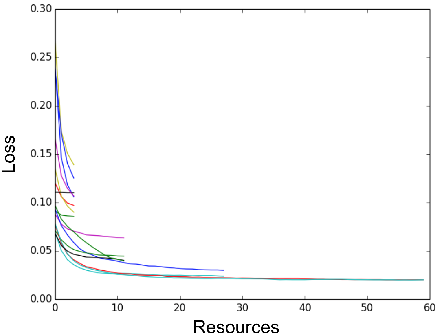
\includegraphics[width=0.9\linewidth]{../w07_hpo_speedup/images/hyperband/Figure_1_2.png}
% \end{figure}
%     \end{column}
%     \end{columns}
%     \begin{columns}
    
%     \begin{column}{.45\linewidth}
%     \vspace{-9em}
%     \begin{itemize}
% 	\item Result: Examine more configurations.
% 	\fhpause
% 	\item Resources:
% 	\fhpause
% 	\begin{itemize}
% 	    \item Runtime
% 	    \fhpause
% 	    \item Number of epochs/iterations
% 	    \fhpause
% 	    \item Number of trees
% 	    \fhpause
% 	    \item Data subset size
% 	    \fhpause
% 	    \item Number of features
% 	    \fhpause
% 	    \item Number of cross validation folds
	    
% 	    \item ...
% 	\end{itemize}
% \end{itemize}
% \end{column}

% \begin{column}{.45\textwidth}

% \end{column}

% \end{columns}

% \end{frame}

% %-----------------------------------------------------------------------

% \begin{frame}{Successive Halving(SH)}
% \begin{columns}

% \begin{column}{.45\textwidth}
% \vspace{-1em}
% \begin{itemize}
%     \item Simple technique
%     \item Assumes promising configurations outperform bad configurations, even early on in the algorithm run.
%     %\item Bandit-based approach to hyperparameter optimization.
%     \fhpause
%     \item Uniformly allocate a budget to a set of configurations.
%     \fhpause
% \end{itemize}
% \end{column}

% \begin{column}{.5\textwidth}
% \begin{figure}
%     \centering
%     \vspace{3em}
%     \only<3>{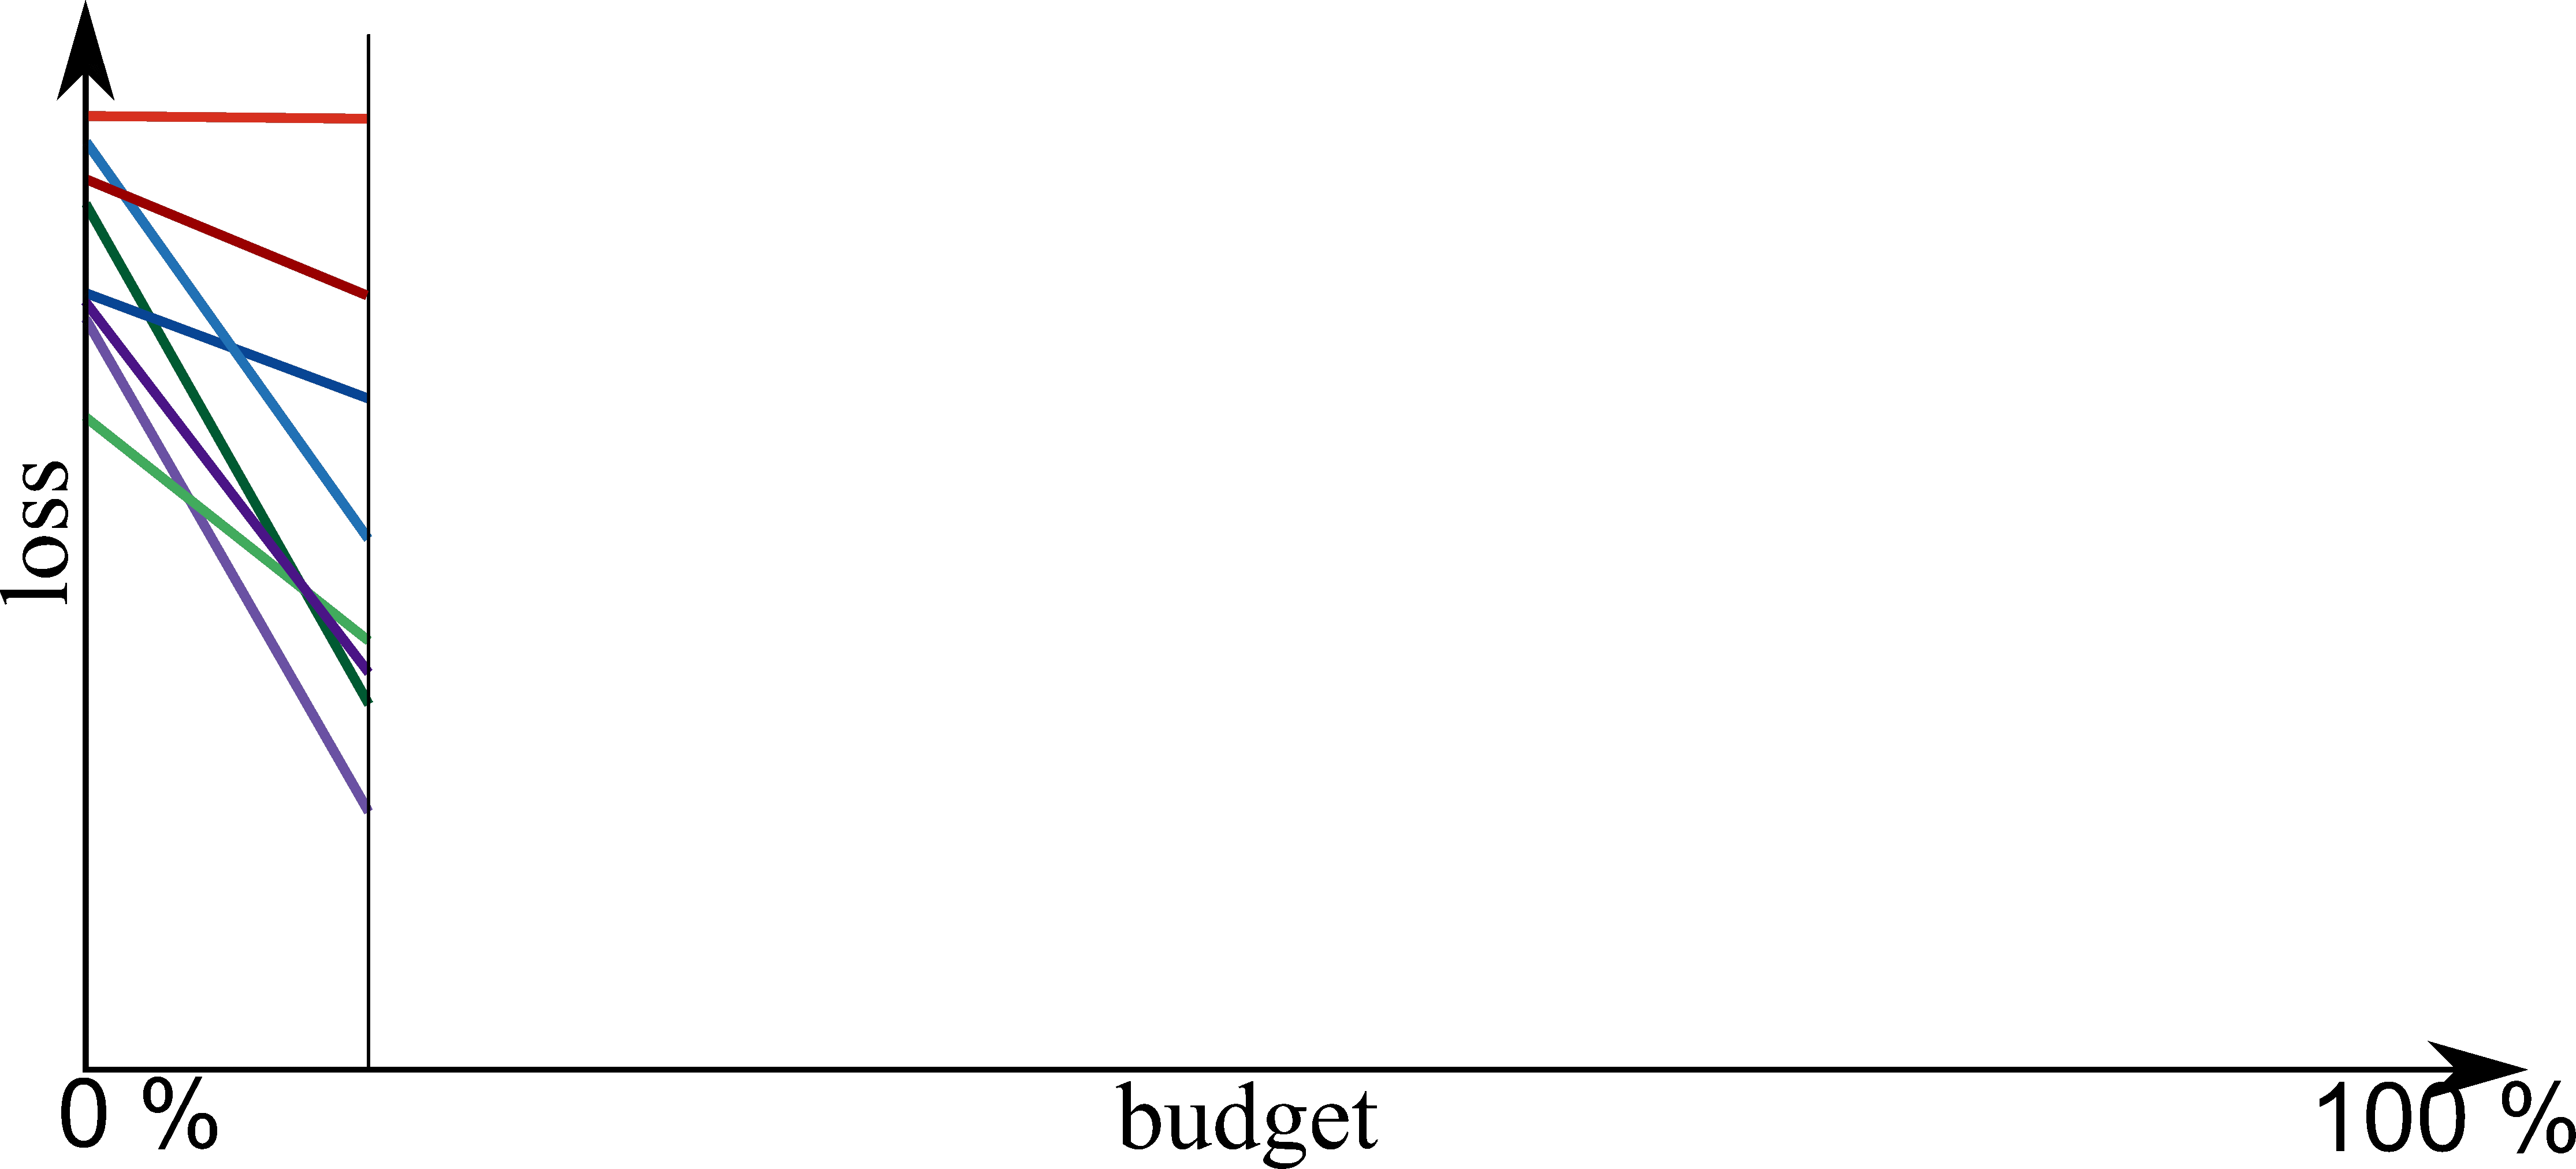
\includegraphics[width=\linewidth]{../w07_hpo_speedup/images/hyperband/SH-1.png}}
%     \only<4>{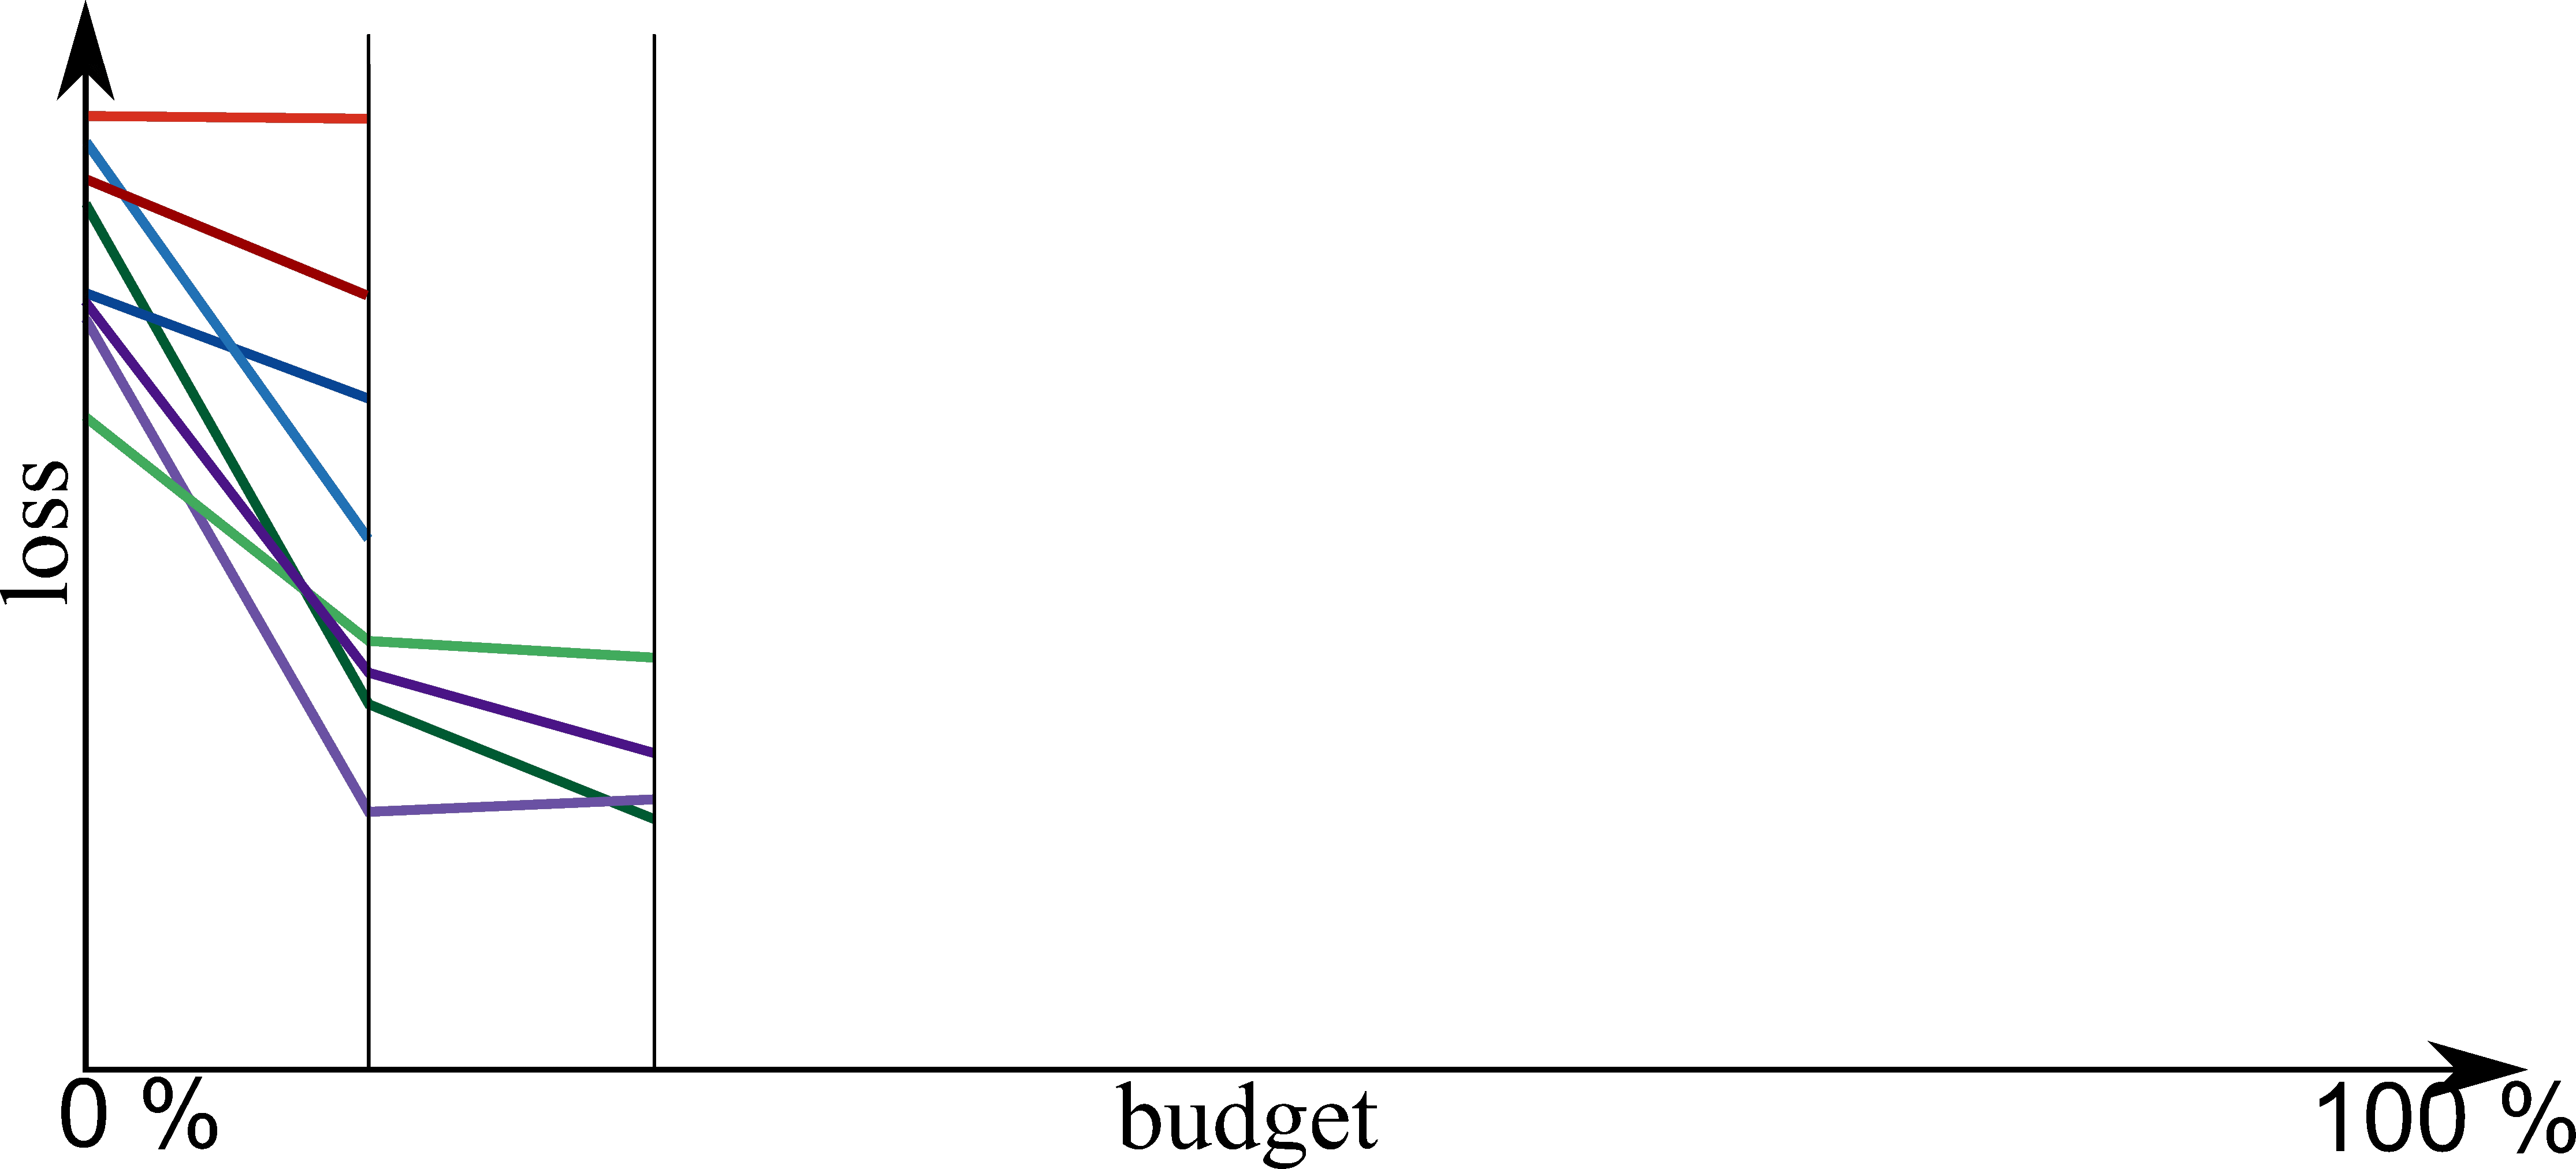
\includegraphics[width=\linewidth]{../w07_hpo_speedup/images/hyperband/SH-2.png}}
%     \only<5>{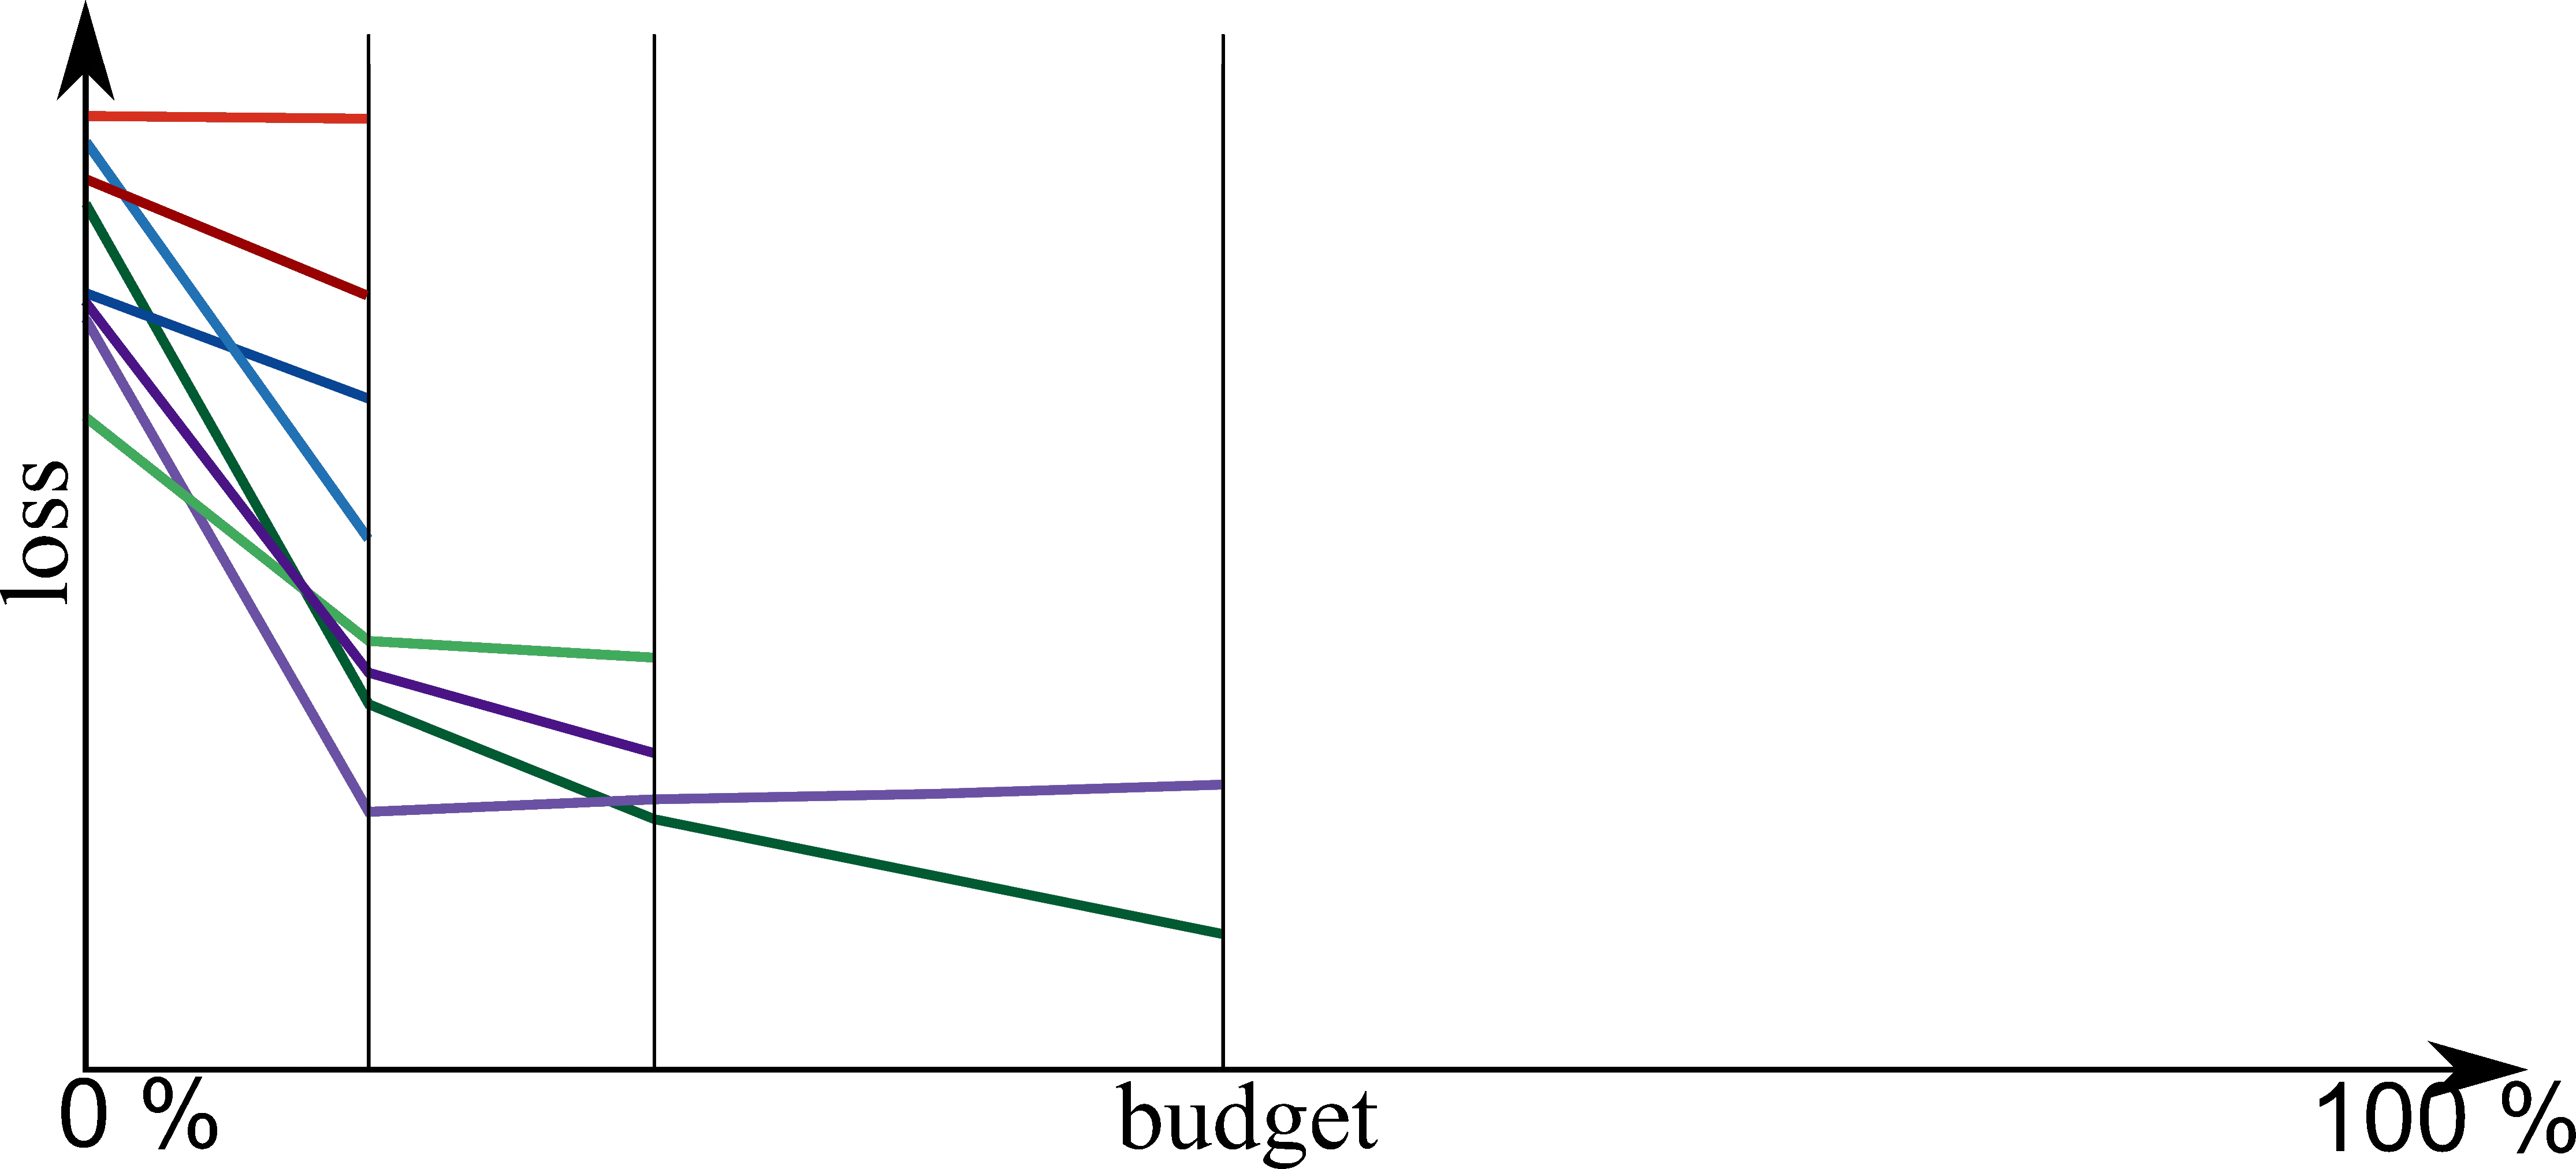
\includegraphics[width=\linewidth]{../w07_hpo_speedup/images/hyperband/SH-3.png}}
%     \only<6>{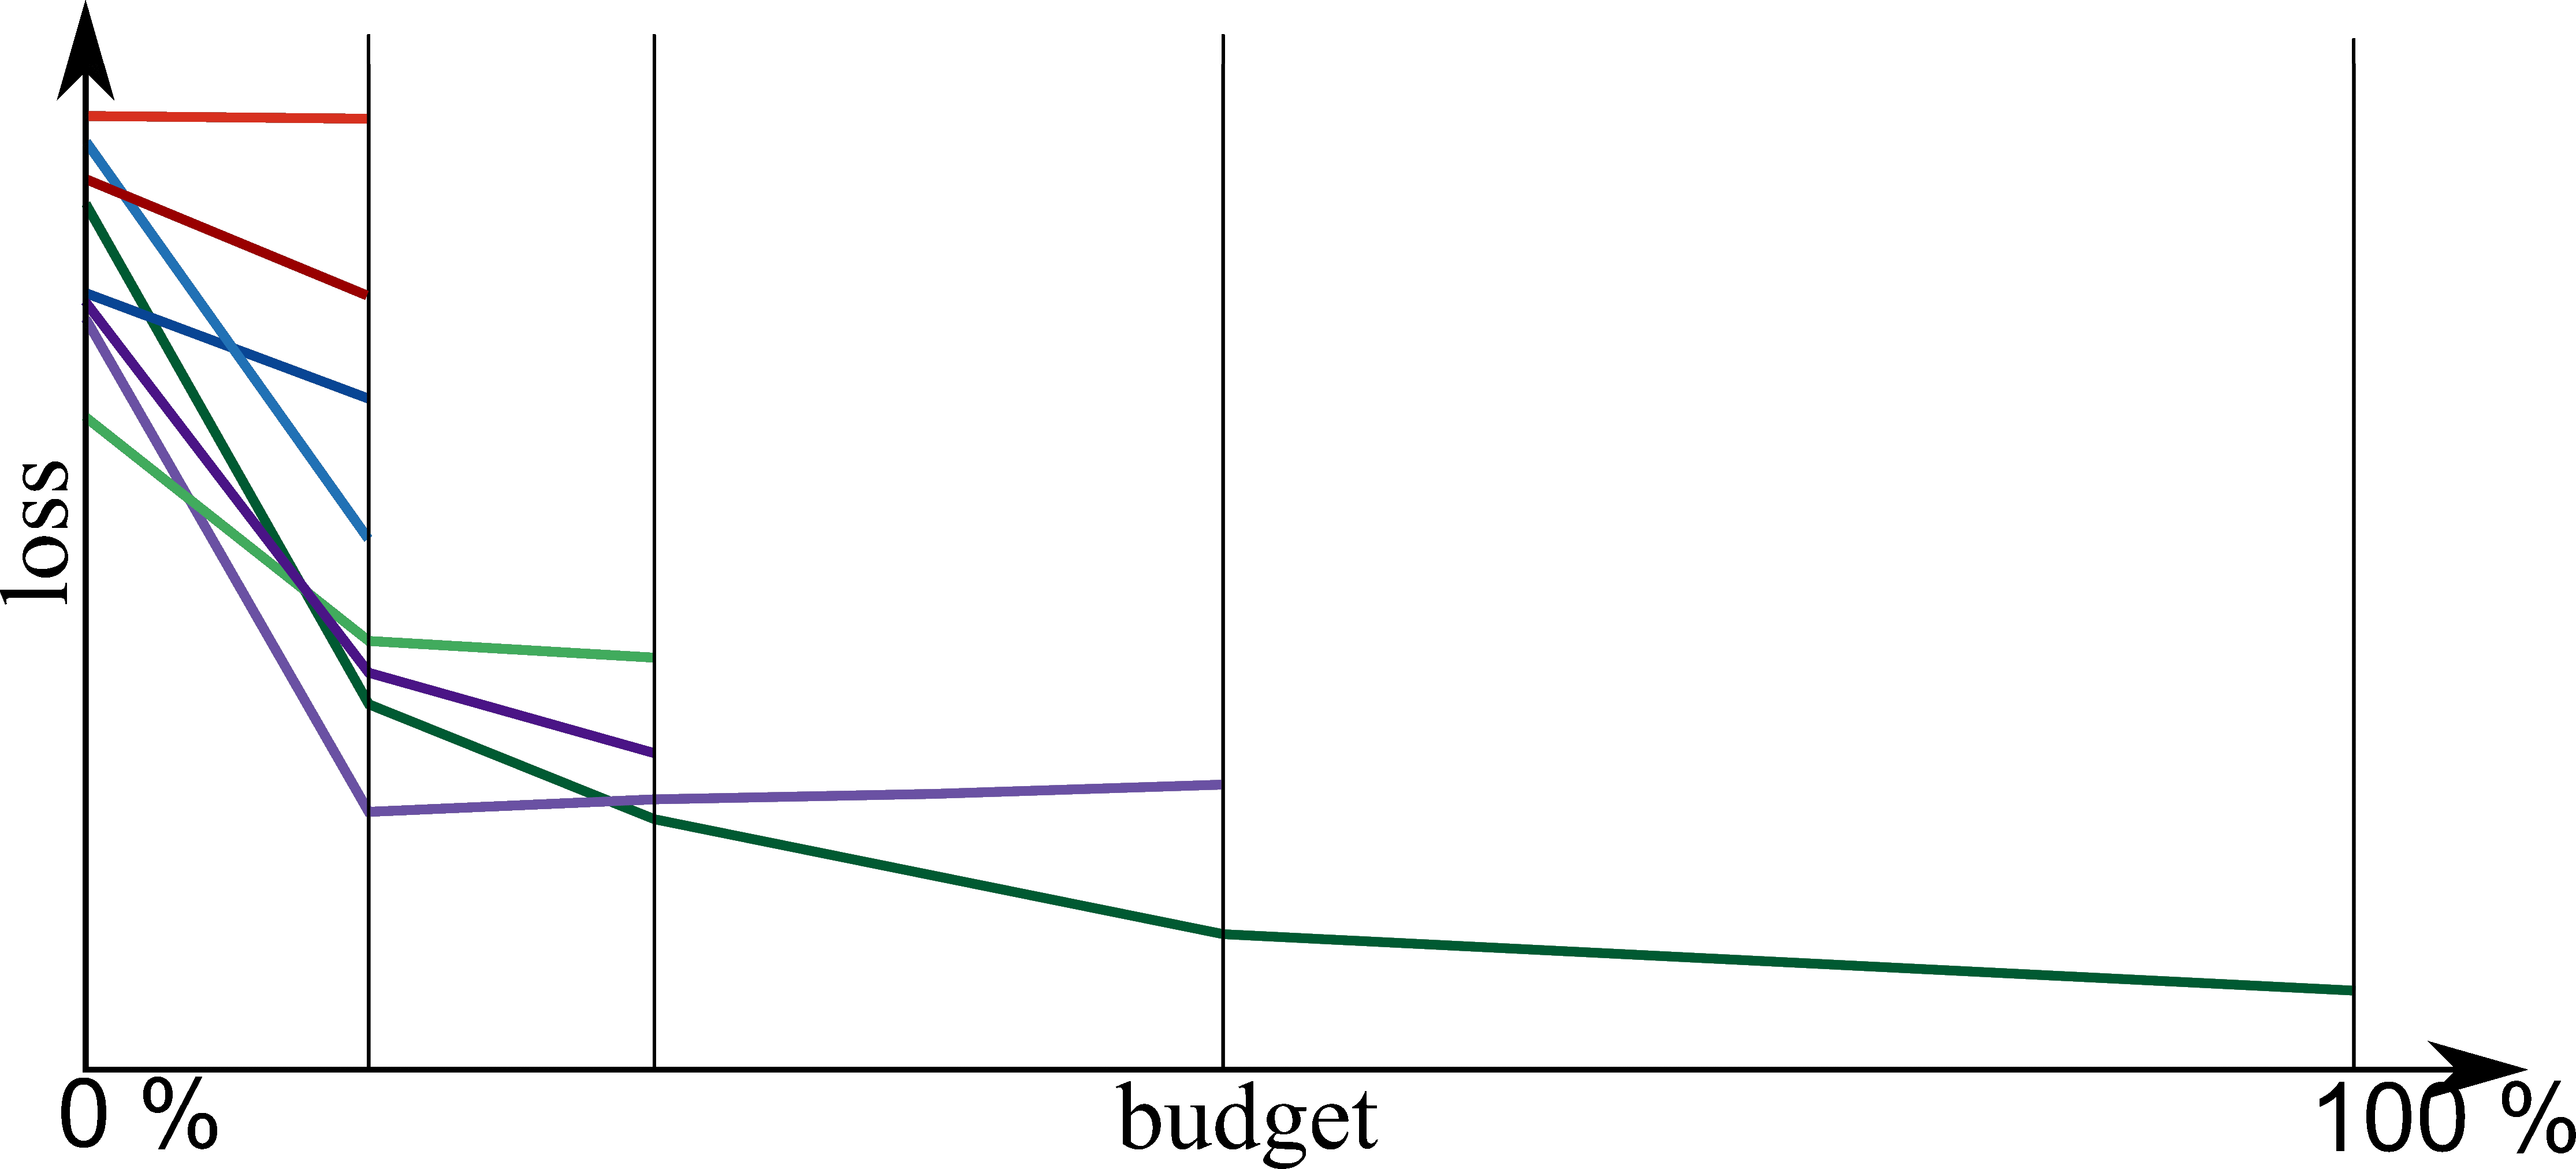
\includegraphics[width=\linewidth]{../w07_hpo_speedup/images/hyperband/SH-4.png}}

% \end{figure}
% \end{column}
% \end{columns}
% \vspace{-5em}
% \begin{columns}
% \begin{column}{.45\textwidth}
% Given a budget $B$ and the number of configurations $n$ as an input:
% \fhpause
% \begin{itemize}
%     \item Evaluate the performance of all configurations.
%     \fhpause
%     \item Drop the worst performing half.
%     \fhpause
%     \item Repeat until termination criterion is met e.g. maximum budget.

% \end{itemize}
% \end{column}

% \begin{column}{.45\textwidth}
% \end{column}

% \end{columns}

% \end{frame}

\begin{frame}{A Simple Multi-Fidelity Algorithms: Successive Halving (SH)}
\vskip -10pt
\hskip 270pt
\lit{\href{http://proceedings.mlr.press/v51/jamieson16.pdf}{Jamieson and Talwalkar, AISTATS 2016}}

\begin{columns}

    \column{0.8\textwidth}
    \begin{itemize}
        \item A very simple algorithm:
        \begin{itemize}
            \item Sample N configurations uniformly at random \& evaluate them on the cheapest fidelity
            \item Keep the best half (or third), move them to the next fidelity
            \item Iterate until the most expensive fidelity (= original expensive black box)
        \end{itemize}
    \end{itemize}
    
    \column{0.2\textwidth}
    \begin{figure}
        \centering
        
\includegraphics[width=0.6\textwidth]{../w07_hpo_speedup/images/hyperband/black_blocks.png}
    \end{figure}

\end{columns}

\begin{figure}
    \centering
    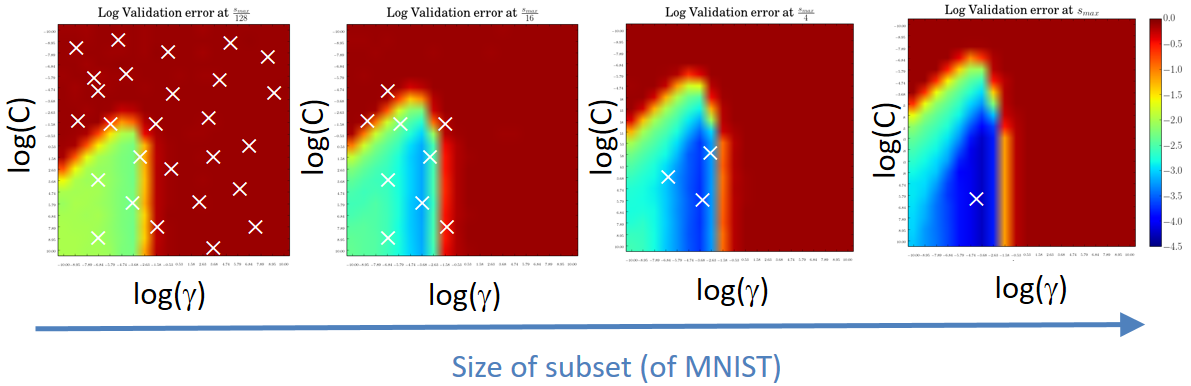
\includegraphics[width=0.8\textwidth]{../w07_hpo_speedup/images/hyperband/hyperband_fidelities.png}
\end{figure}
    
\end{frame}

%-----------------------------------------------------------------------
%-----------------------------------------------------------------------

\begin{frame}{The Same SH Algorithm When the Fidelity is Runtime}
\vskip -10pt
\hskip 270pt
\lit{\href{http://proceedings.mlr.press/v51/jamieson16.pdf}{Jamieson and Talwalkar, AISTATS 2016}}
    
\begin{figure}
    \centering
    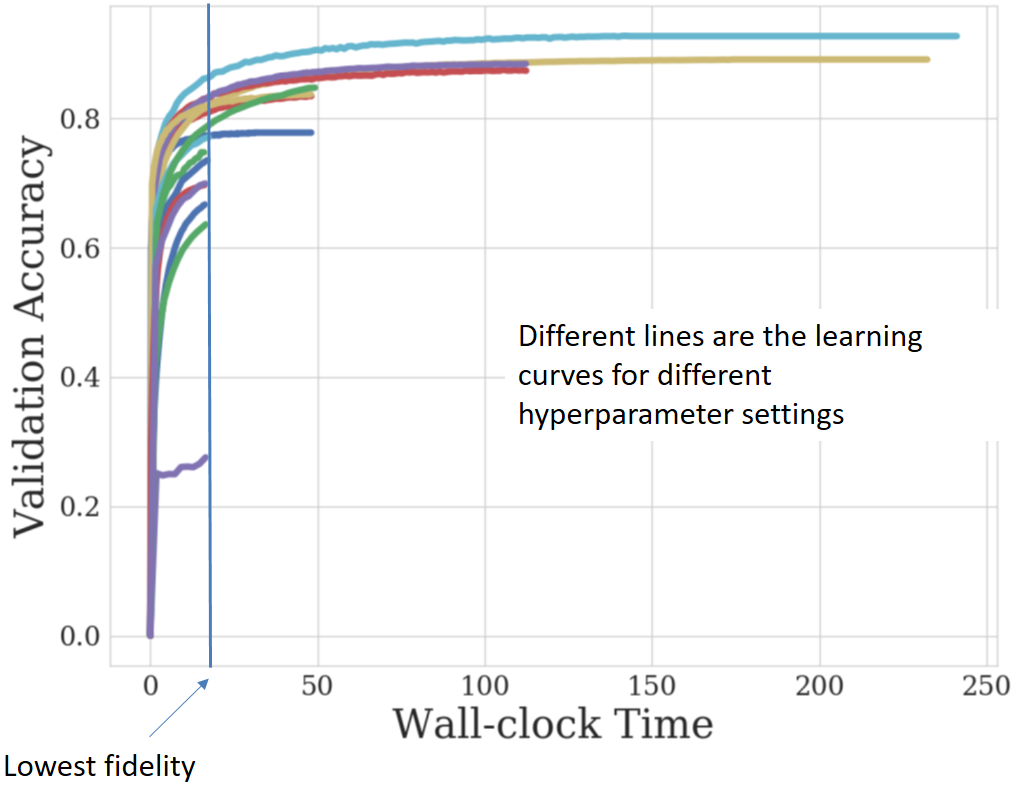
\includegraphics[width=0.6\textwidth]{../w07_hpo_speedup/images/hyperband/sh_accuracy_over_time.png}
\end{figure}
    
\end{frame}

%-----------------------------------------------------------------------
%-----------------------------------------------------------------------

%\begin{frame}{Successive Halving(SH): Algorithm}
%
%\begin{center}
%\begin{minipage}{0.75\textwidth}
%\begin{algorithm}[H]
%    %\DontPrintSemicolon
%    \LinesNumbered
%    \SetAlgoLined
%    \setcounter{AlgoLine}{0}
%    \SetKwInOut{Input}{Input}
%    \DeclarePairedDelimiter\ceil{\lceil}{\rceil}
%    \DeclarePairedDelimiter\floor{\lfloor}{\rfloor}
%    \DeclarePairedDelimiter\abs{\lvert}{\rvert}
%    
%    \Input{ initial budget $b_0,$ maximum budget $b_{max},$ set of $n$ configurations $C=\{\conf_1, \conf_2,\dots, \conf_{n}\}$}
%    $b=b_0$\\
%    \While{$b\leq b_{max}$}{
%    $L=\{\Tilde{\cost}(\conf,b):\conf \in C\}$;\
%    
%    $C=top_{k}(C,L,\lfloor\lvert C \rvert\ / \eta \rfloor)$;\
%    
%    $b=\eta \cdot b$;\
%    }
%    
%    \caption*{Pseudocode for SuccessiveHalving} % used by Hyperband as a subroutine}
%\end{algorithm}
%\end{minipage}
%\end{center}
%\end{frame}
%
%-----------------------------------------------------------------------

%\begin{frame}{\emph{"n versus B/n" Problem}}
%\begin{columns}
%
%\begin{column}{.45\linewidth}
%\begin{itemize}
%    \item SH requires $B$ and $n$ as an input.
%    \item Given finite $B$, $B/n$ resources are allocated across the configurations.
%    \item Configurations need enough minimal resources to differentiate between them in terms of quality.
%\end{itemize}
%\end{column}
%
%\begin{column}{.45\linewidth}
%
%\begin{figure}
%    \centering
%    \vspace{2em}
%    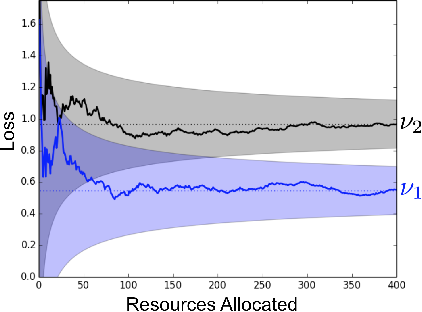
\includegraphics[width=0.9\linewidth]{../w07_hpo_speedup/images/intro/differetiatingConfigurations.png}
%\end{figure}
%\end{column}
%\end{columns}
%
%\vspace{-6.5em}
%\begin{columns}
%
%\begin{column}{.45\linewidth}
%\begin{itemize}
%
%    \item Issue: Optimal allocation strategy is unknown in practice.
%    \item Idea: Perform grid search over a feasible set of tuples of $n$ and minimal resource $r$. (Hyperband) 
%\end{itemize}
%\end{column}
%
%\begin{column}{.45\linewidth}
%
%\end{column}
%    
%\end{columns}
%    
%\end{frame}

% %-----------------------------------------------------------------------
% \begin{frame}{Hyperband}
% \begin{itemize}
%     \item Issue of successive halving (for a fixed B):
%     \begin{itemize}
%         \item Do you want to run many configurations with aggressive rejection?
%         \item Or: Do you want to run few configurations with non-aggressive rejection?
%     \end{itemize}
%     \item Ideas:
%     \begin{itemize}
%         \item Add an outer loop to try different trade-offs between $\#$configurations and budget.
%         \item Add further parameter: proportion of configurations discarded in each round of successive halving
%     \end{itemize}
%     \item Starts with many configurations that gets aggressively rejected.
%     \item In later iterations, fewer configurations with more budget each.
%     \item Returns: configuration with the smallest intermediate loss seen so far.
% \end{itemize}
% \end{frame}

%-----------------------------------------------------------------------

\begin{frame}{An Extension of SH with Theoretical Guarantees: Hyperband}
    
\vskip -10pt
\hskip 330pt
\lit{\href{http://jmlr.org/papers/v18/16-558.html}{Li et al., JMLR 2018}}
    
\begin{columns}

    \column{0.25\textwidth}
    \begin{itemize}
        \item Main Idea: \\ hedge against errors in cheap approximations
\medskip
        \item Algorithm: \\ run multiple copies of SH in parallel, starting at different cheapest fidelities
    \end{itemize}
    
    \column{0.75\textwidth}
    \vskip -20pt
    \begin{figure}
        \centering
        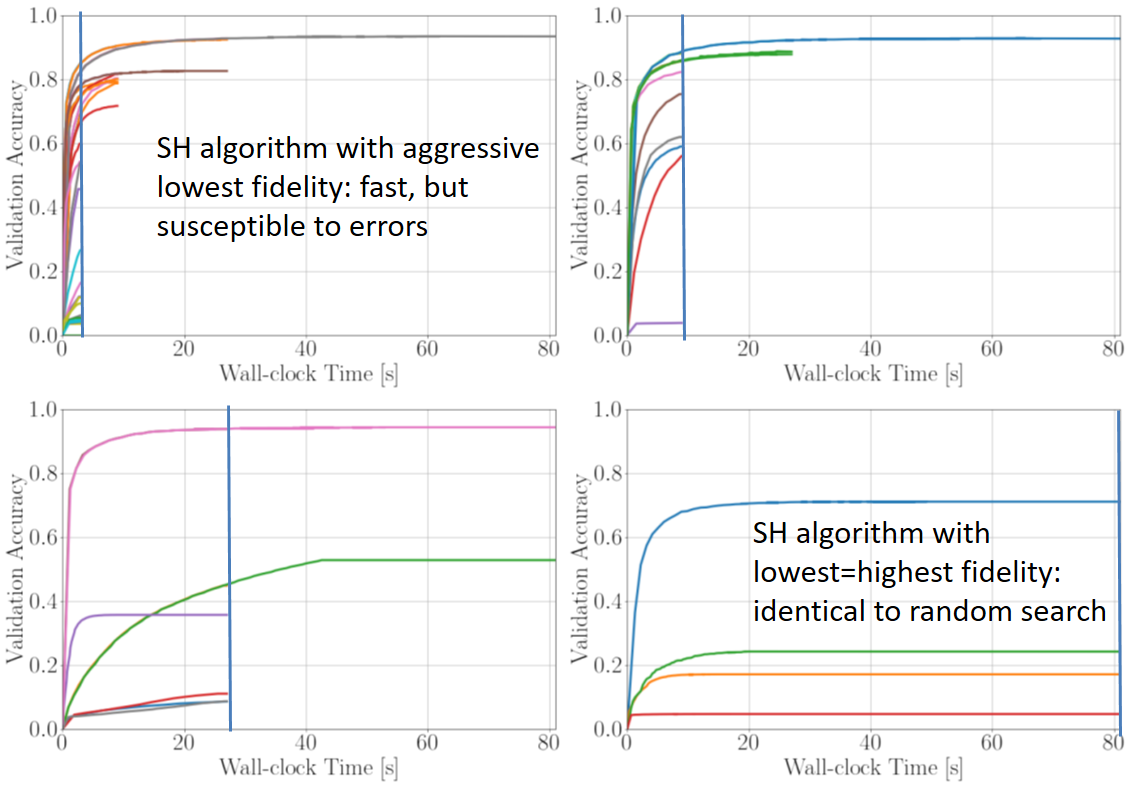
\includegraphics[width=0.9\textwidth]{../w07_hpo_speedup/images/hyperband/hyperband_illustration.png}
    \end{figure}

\end{columns}
    
\end{frame}

%-----------------------------------------------------------------------

%\begin{frame}{Hyperband: Algorithm}
%\begin{center}
%\begin{minipage}{0.75\textwidth}
%\begin{algorithm}[H]
%    %\DontPrintSemicolon
%    \LinesNumbered
%    \SetAlgoLined
%    \setcounter{AlgoLine}{0}
%    \DeclarePairedDelimiter\ceil{\lceil}{\rceil}
%    \DeclarePairedDelimiter\floor{\lfloor}{\rfloor}
%    
%    \Input{budgets $b_{min}$ and $b_{max}, \eta$}
%    
%    $s_{max}=\floor*{\log_{\eta}\frac{b_{max}}{b_{min}}}$;\
%    
%    \For{$s\in \{s_{max}, s_{max}-1, \dots, 0\}$}
%    {
%        sample $\eta=\lceil\frac{s_{max}+1}{s+1} \cdot\eta^{s}\rceil$;\
%        
%        run SH on them with $\eta^{s}\cdot b_{max}$;\
%    }
% 
%        
%    
%    \caption*{Pseudocode for Hyperband using SuccessiveHalving (SH) as a subroutine}
%\end{algorithm}
%\end{minipage}
%\end{center}
%\end{frame}
% %-----------------------------------------------------------------------
% %-----------------------------------------------------------------------
% \begin{frame}{Tradeoffs between n and B/n}
% \vspace{2em}
% \begin{figure}
%     \centering
%     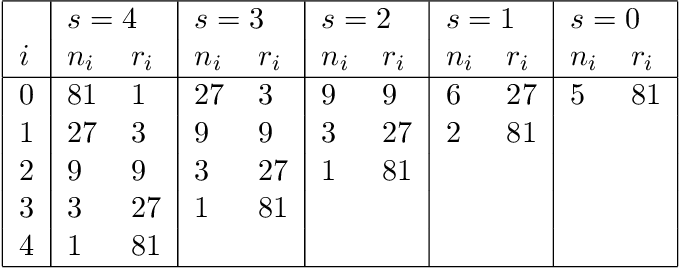
\includegraphics[width=0.7\textwidth]{../w07_hpo_speedup/images/hyperband/Hyperband_Table1-1.png}
%     \caption{The values of $n_i$ and $r_i$ for the brackets of Hyperband corresponding to various values of $s$, when $R = 81$ and $\eta = 3$.}
% \end{figure}

    
% \end{frame}

% %-----------------------------------------------------------------------
% %-----------------------------------------------------------------------
% \begin{frame}{Empirical comparison between individual brackets}
% \begin{figure}
%     \centering
%     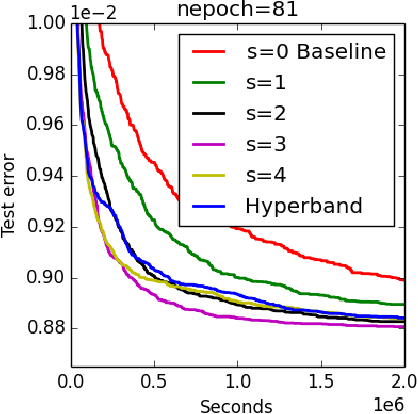
\includegraphics[width=0.4\textwidth]{../w07_hpo_speedup/images/hyperband/Hyperband_figure_3.png}
%     \caption{Performance of individual brackets $s$ and Hyperband.}
% \end{figure}
% \begin{itemize}
%     \item Hyperband is slower than SuccessiveHalving by a small factor if aggressive early-stopping is not suitable for the task.
% \end{itemize}

    
% \end{frame}

% %-----------------------------------------------------------------------
% \begin{frame}{Hyperband: Comparison}
% \begin{figure}
%     \centering
%     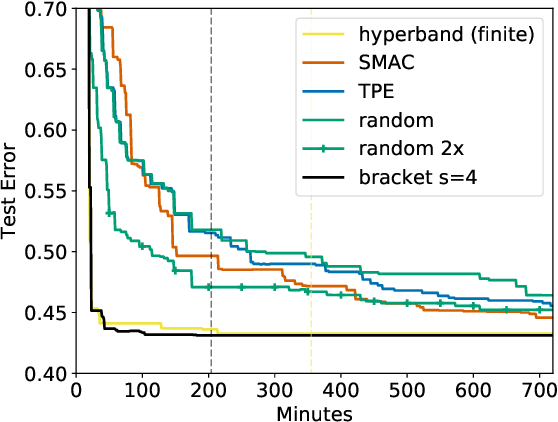
\includegraphics[width=0.55\textwidth]{../w07_hpo_speedup/images/hyperband/Figure_experiments.png}
%     \caption{Average test error of the best kernel regularized least square classification model found by each searcher on CIFAR-10.}
% \end{figure}

    
% \end{frame}

%-----------------------------------------------------------------------

%-----------------------------------------------------------------------
\begin{frame}{Empirical Evaluation: Hyperband vs. Random Search}

\vskip -10pt
\hskip 270pt
\lit{\href{http://proceedings.mlr.press/v80/falkner18a/falkner18a.pdf}{Falkner, Klein \& Hutter, ICML 2018}}

\begin{figure}
    \centering
    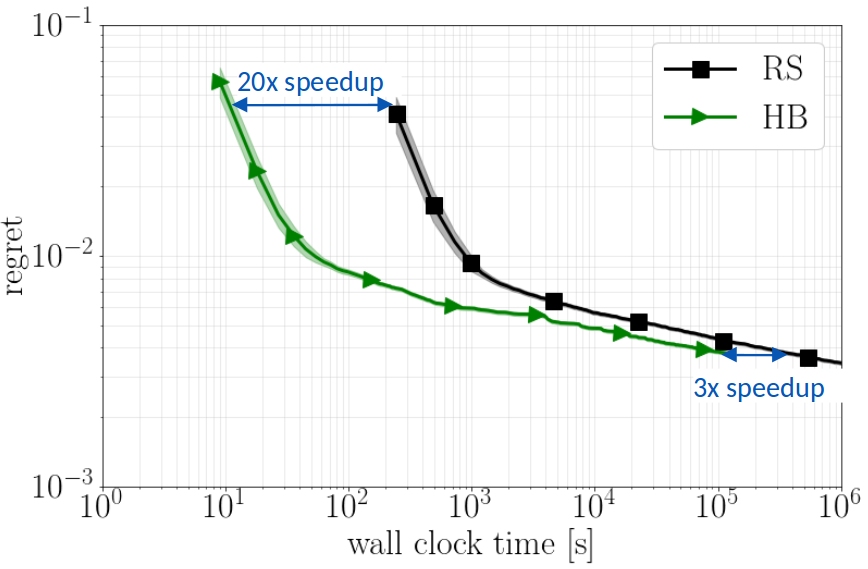
\includegraphics[width=0.7\textwidth]{../w07_hpo_speedup/images/hyperband/bohb_2.png}
\end{figure}

\begin{center}
    Biggest advantage: much improved \emph{anytime performance}
    
    \tiny{Auto-Net on dataset adult}
\end{center}

\end{frame}

%-----------------------------------------------------------------------
%\begin{frame}{Random Search vs. Hyperband}
%
%\begin{itemize}
%   \item In practice HB performs very well for small to medium budgets
%    \item Outperforms random search and vanilla BO
%    \item However, its convergence is limited by its reliance on randomly-drawn configurations
%    \item With larger budgets its advantage over random search diminishes
%\end{itemize}
%\begin{figure}
%    \centering
%    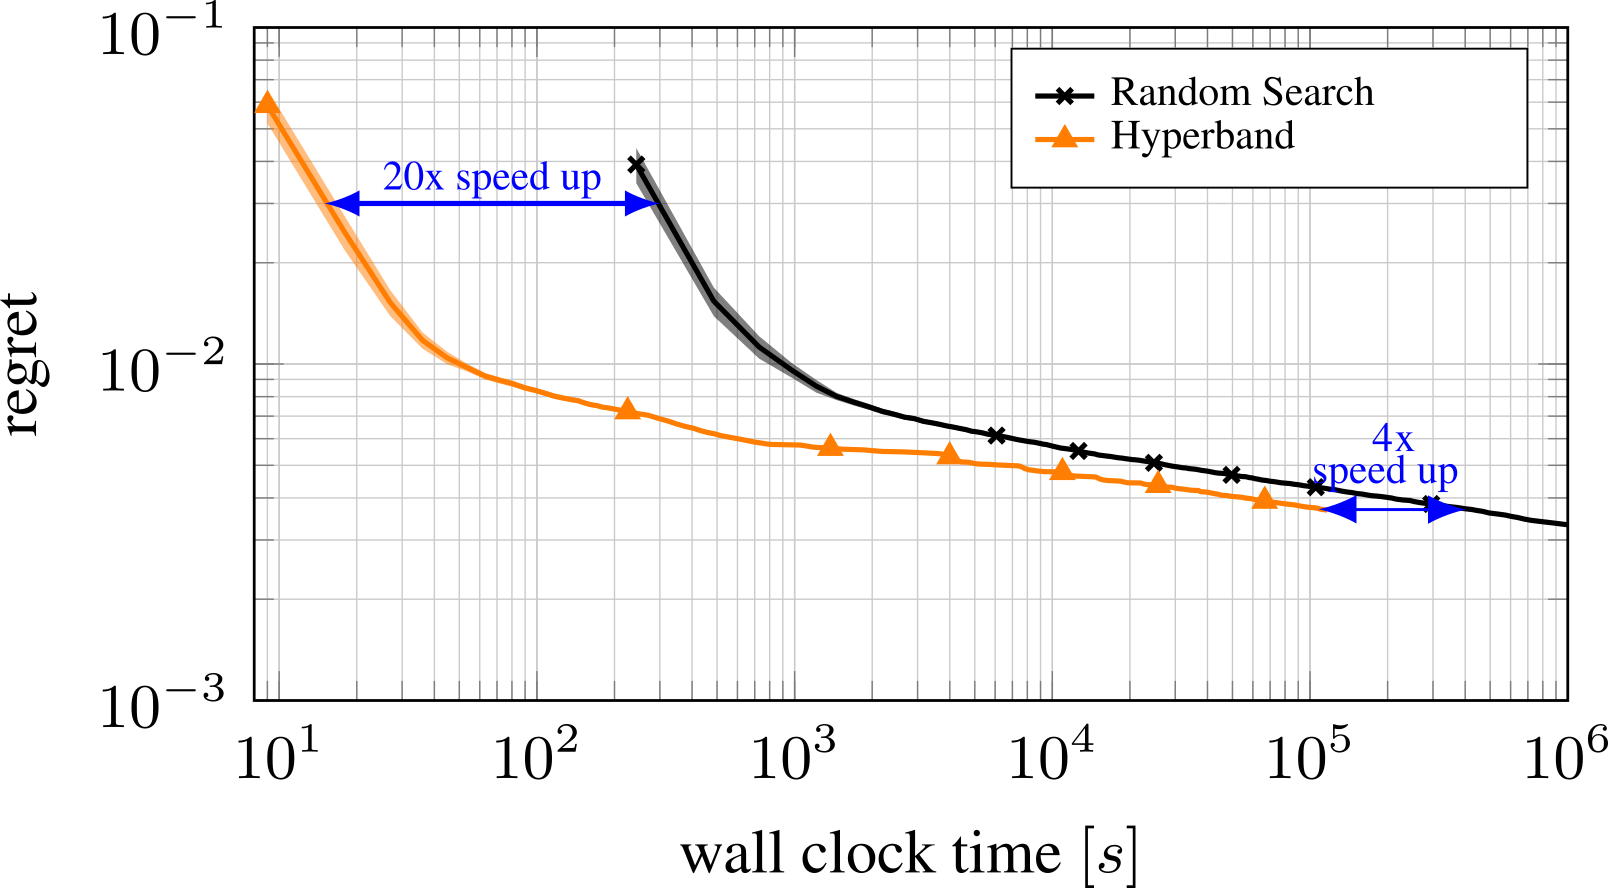
\includegraphics[width=0.6\textwidth]{../w07_hpo_speedup/images/hyperband/comparison_rs_hb.png}
%\end{figure}
%
%
%\end{frame}

%-----------------------------------------------------------------------

%-----------------------------------------------------------------------
\begin{frame}{Questions to Answer for Yourself / Discuss with Friends}

\bigskip

\begin{itemize}
%    \item \alert{Repetition.} Why can't one simply use both a large $B$ and $n$ for doing hyperparameter optimization?

%\medskip
    \item \alert{Discussion.} 
    How do you think Hyperband would compare to successive halving using the most aggressive fidelity?
\medskip    
    \item \alert{Discussion.} How slow is Hyperband in the worst case?

\end{itemize}

\end{frame}
%----------------------------------------------------------------------
%----------------------------------------------------------------------